\documentclass[10pt,twocolumn,letterpaper]{article}

\usepackage{statcourse}
\usepackage{times}
\usepackage{epsfig}
\usepackage{graphicx}
\usepackage{amsmath}
\usepackage{amssymb}

% Include other packages here, before hyperref.

% If you comment hyperref and then uncomment it, you should delete
% egpaper.aux before re-running latex.  (Or just hit 'q' on the first latex
% run, let it finish, and you should be clear).
\usepackage[breaklinks=true,bookmarks=false]{hyperref}


\statcoursefinalcopy


\setcounter{page}{1}
\begin{document}


%%%%%%%%%%%%%%%%%%%%%%%%%%%%%%%%%%%%%%%%%%%%%%%%%%%%%%%%%%%%%%%
% DO NOT EDIT ANYTHING ABOVE THIS LINE
% EXCEPT IF YOU LIKE TO USE ADDITIONAL PACKAGES
%%%%%%%%%%%%%%%%%%%%%%%%%%%%%%%%%%%%%%%%%%%%%%%%%%%%%%%%%%%%%%%



%%%%%%%%% TITLE
\title{NLP Project Proposal: Classifying Newspaper \\ Political Bias with Domain-Context augmented Transformers}

\author{Tom Arend\\
{\tt\small t.arend@phd.hertie-school.org}
\and
Nicolai Berk\\
{\tt\small nicolai.berk@gmail.com}
}

\maketitle
%\thispagestyle{empty}


% MAIN ARTICLE GOES BELOW
%%%%%%%%%%%%%%%%%%%%%%%%%%%%%%%%%%%%%%%%%%%%%%%%%%%%%%%%%%%%%%%

\begin{abstract}
    Newspapers are one of the most important institutions influencing political outcomes in contemporary democracies. They have the power to affect voting behaviour \cite{Chiang2011, Ladd2009}, as well as polarise the electorate \cite{Lelkes2017} or motivate them to turn out to vote \cite{Gentzkow2010}. Therefore, it is surprising that few papers deploy state-of-the-art Deep Learning technologies to classify ideological bias in news articles. We first fine-tune a transformer neural network on party press releases, which we subsequently augment with domain-relevant contextual data, before we go on to estimate ideological bias in news articles. We proceed to compare both models to an ambitious baseline model and prior accuracy scores in the literature.
\end{abstract}

%%%%%%%%% BODY TEXT


\section{Introduction}

Political scientists often want to classify texts into categories based on their content. For example, a researcher might want to classify congressional speeches based on their ideological content, or find out whether political speeches invoke nationalist themes, or even classify news articles based on the narratives they use (Krebs 2015). As many of the issues contained within politicians' speeches are so nuanced that even word choice can convey policy positions, it is unsurprising that most of the efforts are centered around identifying ideological components of speeches, press releases and campaign adverts. Newspapers, or more precisely editorials themselves have received comparatively less attention. Yet they are one of the most influential institutions influencing political outcomes in contemporary democracies. \footnote{Here is the github repository that we will be using for the project: \href{https://github.com/nicolaiberk/nlpdl\_project}{https://github.com/nicolaiberk/nlpdl\_project}} \\

Newspaper have the power to affect voting behaviour, as well as polarise the electorate or motivate them to turn out to vote. While the impact of political news media has often been studied, their political bias has usually been assumed a-priori. To improve our understanding of the effects of news medias' ideological bias, it is important to understand how this bias compares across time and space. A number of studies have drawn on NLP and state-of-the-art Deep Learning techniques to automatically classify and identify newspaper slant. However, the existing models tend to (for the most part) ignore domain knowledge inherent to political science to improve the classification of newspaper slant. \\

We aim to address this shortcoming in the literature by putting forward a transformer neural network augmented with contextual information to beat state-of-the art classifiers. We aim to achieve this by fine-tuning an existing pre-trained model (either BERT, RoBERTa, DistilBERT or XLNet) on political texts and then using this model to identify newspaper biases. In a first phase, we intend to fine-tune an already pre-trained model on party press releases, using contextual information to supplement it. In a second phase we apply this model to classify newspaper bias. We compare both models to an ambitious baseline model using BERT. Estimates are validated using a number of technical tests and a comparison with previous findings in the literature. \\

\section{Related Work}

Measuring ideology is the prime use-case of automated text analysis in political science. While some work has used supervised learning to understand political polarisation \cite{Ash2017} as well as media slant \cite{Widmer2020}, this existing work estimates the polarisation of political actors or newspapers across time, or simply the similarity of one news source to others. Existing models have for the most part relied on bag-of-words approaches, including the scaling of texts using supervised \cite{Laver2003} or unsupervised models \cite{Slapin2008}. Unsurprisingly, the performance of these models has so far proven unreliable, lagging behind the accuracy of human coders or expert judgement \cite{Brauninger2013, Hjorth2015, Koljonen2020}. Recent applications have assessed the ability of deep learning models to replicate human coding of party manifestos \cite{Bilbao-Jayo2018} or estimate ideology directly using supervised classification \cite{Simoes2020}. These applications employ RNNs or CNNs. We feel they could be improved upon with state-of-the-art transformer neural networks.\\

Much less work has been devoted to the measurement of the ideological leaning of newspapers. While some work has assessed the impact of endorsements of specific candidates \cite{Chiang2011, Ladd2009}, there have been few attempts to scale newspapers on ideology. Gentzkow and Shapiro estimate slant in US newspapers by identifying bi- and trigrams' indicative of a congressional speakers' party, and apply the resulting dictionary to newspapers to scale them \cite{Gentzkow2010}. More recently, Widmer et al. have assessed polarisataion in the US media environment using a supervised model. They train a classifier on bigrams, predicting whether content was produced by a left-leaning network (CNN) or a right-leaning network (Fox news) \cite{Widmer2020}. \\

We believe both approaches are likely inferior to more complex deep learning models, as such novel approach would not incorporate idiosyncratic phrases used by the specific networks identified to train the data. Using party labels to train classifiers is more straightforward, as it places newspapers within the existing context. However, any algorithm trained on a different dataset than applied to must be subject to careful validation.\\


\section{Motivation}

To our best knowledge, newer Sequence-to-sequence models have so far not been applied to the classification of newspaper biases. Beyond the implicit motivation inherent to such a research gap, we fundamentally believe that providing a state-of-the-art model to identify ideological biases in newspapers is also beneficial to the wider political science discipline and real-world applications alike. \\

As stated-above, newspapers are an important institution in the analysis of political phenomena, ranging from polarization to voter turnout. If the existing approaches to classify newspaper slant can be approved upon, or even just complemented, we could provide an additional tool for researchers to study the impact of newspaper slant. A working state-of-the-art model might even renew interest in the subject matter and encourage researchers to find new and exciting applications for it. \\

Outside of academia, a confident and robust classifier of newspaper bias, might help readers identify when they are reading an article that is overly partisan. This would perhaps encourage them to approach certain news sources with more scepticism and hold news outlets to higher editorial standards. In the long run, the highlighting of biases in articles might counteract the worrying polarization of entire electorates. \\

On a more personal note, the chosen project would also align with an area that both authors have a substantive research interest in. It is this combination of domain knowledge with cutting edge technical approaches that provides ample motivation to conduct this project.\\

\section{Evaluation}

We believe that there will be two separate aspects to the evaluation of the project. The first aspect derives from the personal gain (in an educational sense) that we would like to take away from this project. The second aspect contains the technical robustness and accuracy of the model we train. 
\begin{enumerate}
    \item This concerns the successful training and validation of a state-of-the-art deep learning model for NLP. Since neither of the authors have experience in setting up neural networks, we would consider the baseline for personal success in setting up a valid model that would hold up to the scrutiny of our peers. Evidently, we are more ambitious than that and are hoping to train a number of these models in order to select the most accurate of them. In this way we would hope to gain an advanced level of knowledge of deep learning approaches for NLP that could eventually lead to real and concrete applications in our respective sub-fields of political science.
    \item To measure the technical success of our project, we aim to deploy the standard approach in the literature. In order to evaluate the proposed approach, the dataset will be divided into two different subsets: training and validation sets (85\%), and a test set (15\%) on which we will measure the accuracy of our model. The model may overfit with respect to the validation set. Therefore, a third set, the test set, will be used in order to measure the real performance of the model. Subsequently we will present two statistics that represent the validity of our model; the accuracy rate and the F-measure/test. The current state-of-the-art seems to approach an accuracy of 65-70\% \cite{Devlin2019}. Should our model come close to this score, we would consider the project a success. The best case scenario would be if we could improve on this score by several percentage points.
\end{enumerate}
 

\section{Resources}

The project will employ the following German language datasets:
\begin{enumerate}
    \item To fine-tune our transformer model, we intend to employ political texts in the form or party press releases from Germany that cover the years from 2015-2020. They are labelled with party information and the ideological orientation of that party. This data was collected by the authors for previous projects.
    \item The dataset of newspaper articles that will be classified according to their ideological bias, is in the process of being collected. Though we are looking into already existing alternatives. All newspaper articles are scraped from the online archives of the main daily newspapers in Germany. 
\end{enumerate}

One of the remaining open questions concerns the the language of our datasets. For now, they are only in German. We found contradicting evidence only suggesting that certain mono-lingual pretrained models suffer compared to multilingual pretrained models. We were thus wondering whether we ought to expand the collection of datasets to include English-language political data, such as the e Ideological Books Corpus (IBC), which was compiled by a group of researchers from the University of Maryland \cite{sim-etal-2013-measuring}. If that were necessary, we could apply our model to a dataset of English-language newsarticles, such as the Media Bias Annotation Dataset \cite{Spinde2021MBIC} or the slant newspaper data by Gentzkow and Shapiro \cite{Gentzkow2010}. \\

We will use our individual personal laptops to conduct the training and validation of the model. However, the authors will take advantage of the free computational resources that are available through Google Colab. \\

\section{Contributions}

Since our group consists of two people we fully intend to divide to workload equally among us. In the following section we will details specifically which task each of us will accomplish. \\

\textbf{Writing Tasks:}
\begin{itemize}
    \item The idea for the project was elaborated in concert in a number of online meetings.
    \item Whereas Tom did the majority of the writing for the proposal, Nico researched some prior work, set up the group's github account, and collected guides to facilitate the technical collaboration on that platform. 
    \item We expect that Nico will take over most of the writing duties for the midterm progress report.
    \item The final report will be written in equal parts by both authors. Each will contribute the section on which he worked most. (If Nico conducted the majority of the accuracy tests, he will write the section on validity etc.)
\end{itemize}

\textbf{Computational Tasks:}
\begin{itemize}
    \item We expect to contribute equally to the training and validation of the model. 
    \item For now, both of us have experimented with existing data, but the exact separation of tasks will be established once we have progressed a little further in the course. This will hopefully give us a clearer idea on how to identify and structure the necessary computational tasks to successfully complete our project.
\end{itemize}


{\small
\bibliographystyle{ieee}
\bibliography{proposal.bib}
}

\end{document}




When discussing related work, do not forget to include appropriate references.  This is an example of a citation \cite{kim_convolutional_2014}. To format the citations properly, put the corresponding references into the bibliography.bib file. You can obtain BibTeX-formatted references for the "bib" file from Google Scholar (\url{https://scholar.google.com}), for example, by clicking on the double-quote character under a citation and then selecting \mbox{"BibTeX"} as shown in Figure \ref{fig:google-scholar-1col} and Figure \ref{fig:google-scholar-2col}.


\begin{figure}[t]
\begin{center}
   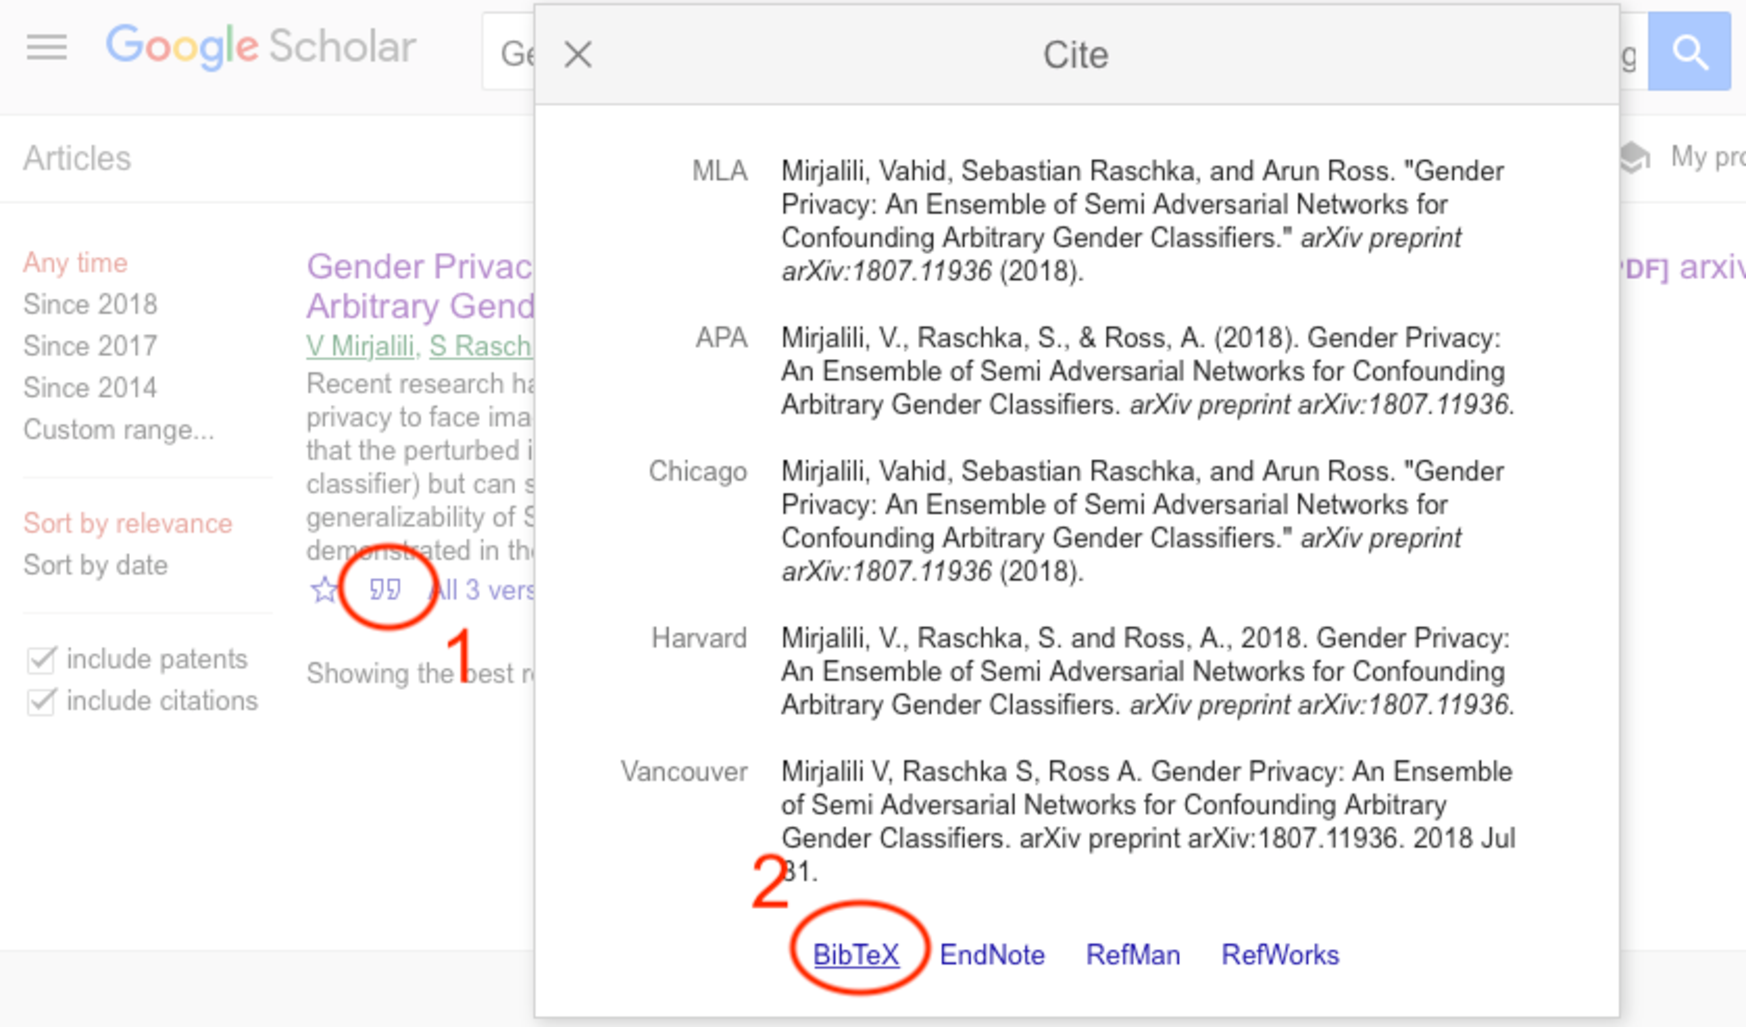
\includegraphics[width=0.8\linewidth]{figures/google-scholar.pdf}
\end{center}
   \caption{Example illustrating how to get BibTeX references from Google Scholar as a 1-column figure.}
\label{fig:google-scholar-1col}
\end{figure}


\begin{figure*}
\begin{center}
   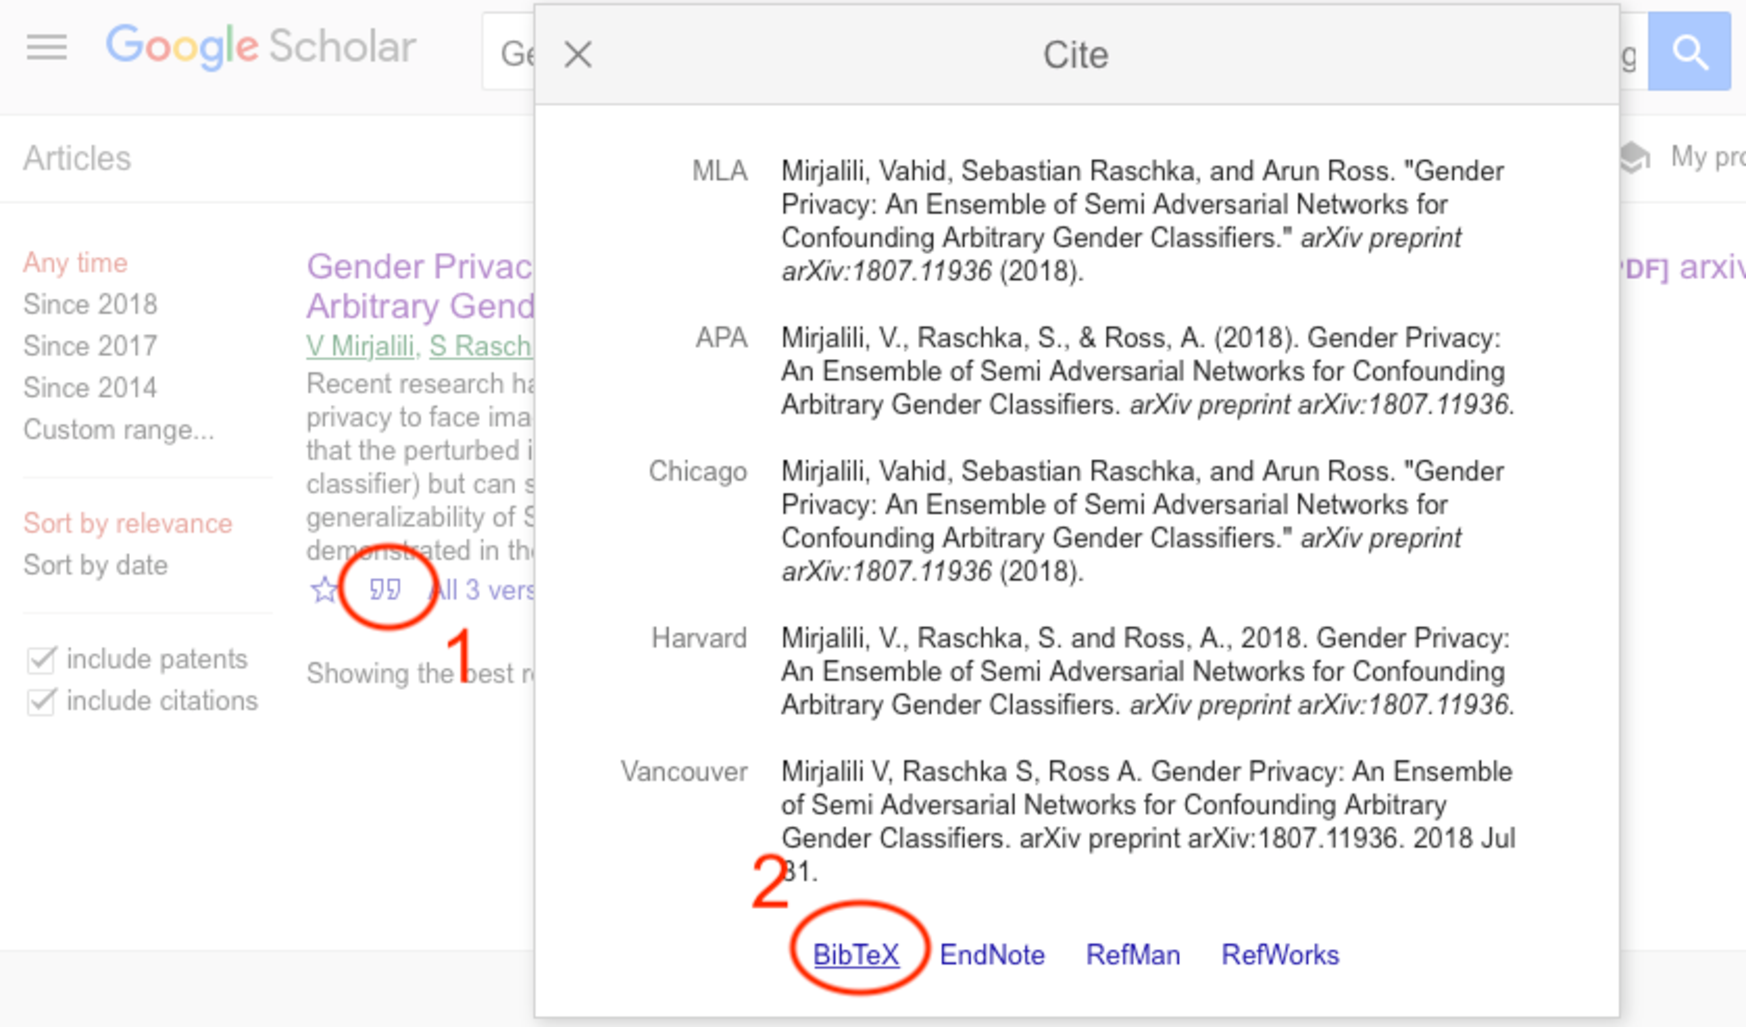
\includegraphics[width=0.8\linewidth]{figures/google-scholar.pdf}
\end{center}
   \caption{Example illustrating how to get BibTeX references from Google Scholar as a 2-column figure.}
\label{fig:google-scholar-2col}


\end{figure*}